\documentclass[11pt,a4paper]{report}
\usepackage[utf8]{inputenc}
\usepackage[french]{babel}
\usepackage[T1]{fontenc}
\usepackage{amsmath}
\usepackage{amsfonts}
\usepackage{amssymb}
\usepackage{graphicx}
\begin{document}
\begin{titlepage}
\newcommand{\HRule}{\rule{\linewidth}{0.5mm}}
\center
\textsc{\LARGE
Ecole Nationale Superieure Polytechnique de Maroua
} \\[1cm]
\textsc{\Large
Departement d'Informatique et Telecommunications
} \\[1cm]
\textsc{\large
\underline{UE} : Cryptographie avancee \\ \underline{CODE} : SEC519
} \\[1cm]
\HRule \\[0.4cm]
{ \huge \bfseries Rapport des Travaux Diriges 1  \\[0.15cm]}
\HRule \\[1.5cm]
KOUAM CHEKAM LEOPOLD JUNIOR \\
18A0265P \\[1cm]
MOGO KAMDEM ROOSEVELT\\
18A0308P \\[1cm]
\today \\ [1cm]
\end{titlepage}
\newpage
\tableofcontents
\chapter*{Introduction}
\chapter{Étude de l'existant}
\chapter{Cahier de charge}
\section{Contexte et définition du problème}
 Dans le cadre de l'unité d'enseignement Spécialisation en cryptographie 2, nous nous sommes intéressé à la manière donc les personnes et entreprises gèrent leurs mots de passe mais surtout à la robustesses de ceux-ci.
 \section{Objectifs du projet}
 Dans le but de faciliter la gestion des mots de passes aux utilisateurs/entreprises, nous avons opté concevoir et produire une solution de gestion de mot de passe robuste.
 \section{Spécifications des besoins}
 \subsection{Besoins fonctionnels}
 Il est question pour nous dans cette section de définir les besoins fonctionnels de notre gestionnaire de mot de passe.un besoin fonctionnel est un action ou un comportement permis dans le système. Notre système permettra :
 \subsubsection{Cas d'utilisation personnel}
 \begin{itemize}
 \item Authentifier un utilisateur
 \item Ajouter/Modifier/Supprimer un mot de passe
 \item generer un mot de passe robuste
 \item tester la robutesse d'un mot de passe
 \end{itemize}
 
 \subsubsection{Cas d'utilisation en entreprise}
 \begin{itemize}
 \item Authentifier un utilisateur
 \item Authentifier un client
 \item Ajouter/Modifier/Supprimer un mot de passe
 \item Ajouter/Modifier/Supprimer un client
 \item Donner des droits de lecture/ecriture sur un mot de passe a plusieurs utilisateurs
 \item generer un mot de passe robuste
 \item tester la robutesse d'un mot de passe
 \end{itemize}
 
 \subsection{Besoins non fonctionnels}
 un besoin non fonctionnel est un exigence propre au système niveau performance, matériel ... mais surtout les contraintes d'implémentation. Ainsi le système doit :
 \begin{itemize}
 \item simple a utiliser
 \item un délai de réponse très court
 \item fonctionner suivant l'architecture client-serveur (trois niveaux) 
 \item évolutif
 \end{itemize}
 \subsection{Méthode et outils utilisee}
  Le projet
\chapter{CONCEPTION ET Implémentation}
\section*{Introduction}
 Pour la realisation de notre projet, sa conception et modelisation est une etape crucial.Nous presenterons dans ce chapitre la modelisation detaille de notre systeme mais aussi son implementation appuye des differentes technologies utilisees.
 
 \section{Conception et Modelisation}
 \subsection{Outils de Modelisation}
 \begin{itemize}
 \item StarUML
 \item draw.io
 \end{itemize}
 \section{Diagramme de Cas d'utilisation}
 \subsection{Les Acteurs du Systeme}
 Nous entendons par acteurs l'ensemble des outils ou personnes qui interagissent avec notre systeme. Nous pouvons citer entre autres:
 \begin{itemize}
 \item L'administateur : C'est le gerant de notre systeme.
 \item Le Client : C'est un service qui sera connecte a notre application
 \item l'utilisateur : c'est le proprietaire des differents mots de passe sur chacun des services
 \end{itemize}
 \subsection{Cas d'utilisation general}
 La figure presente le diagramme de cas d'utilisation general de notre systeme.
 \begin{center}
 \begin{figure}[!h]
 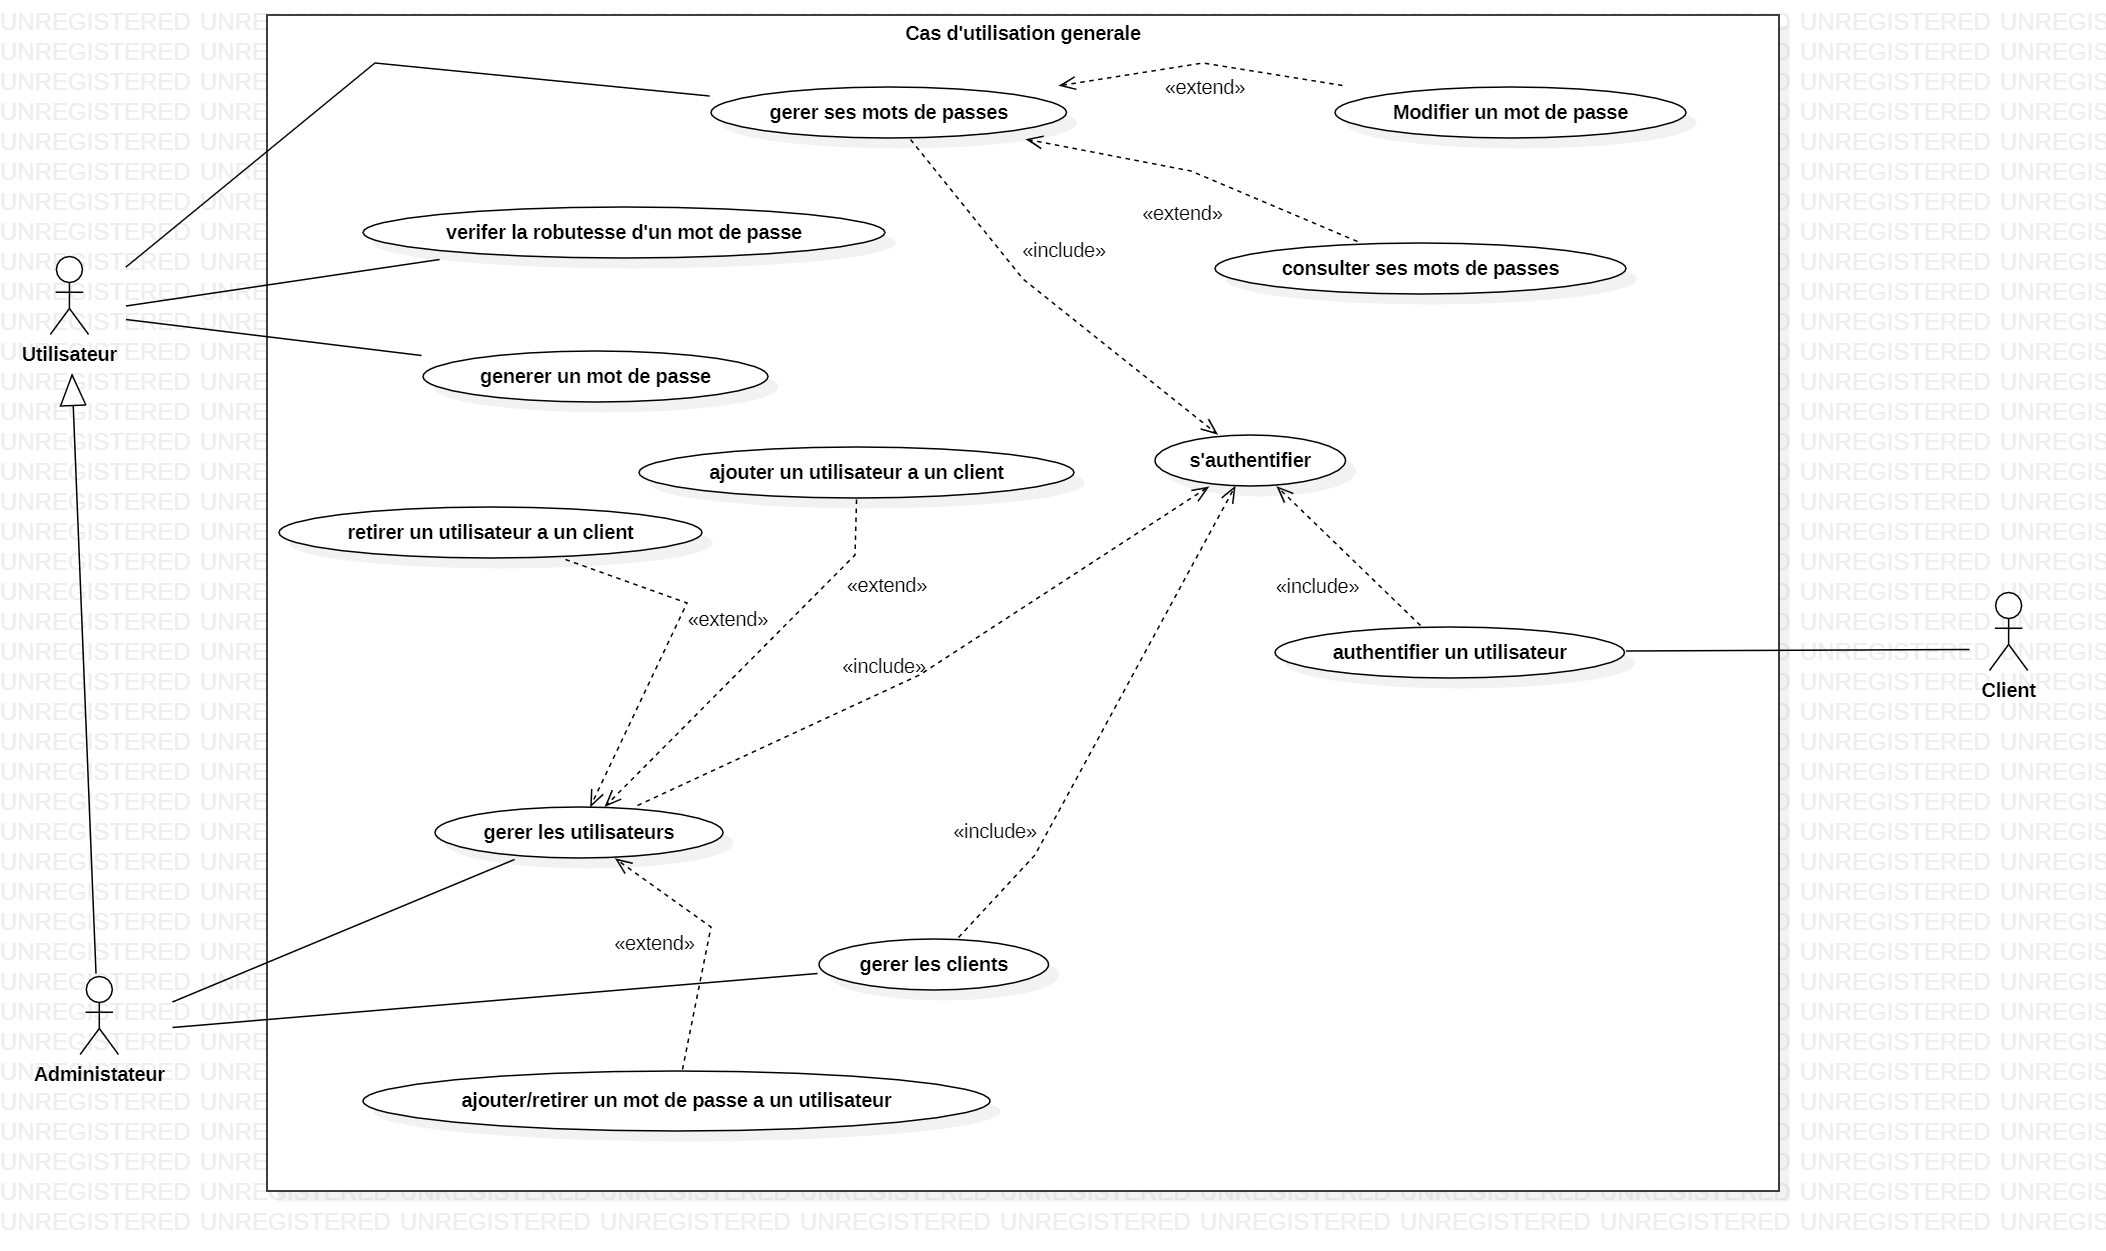
\includegraphics[scale=0.2]{img/casutilisationgeneral}
 \caption{Cas d'utilisation general}
 \end{figure}
 \end{center}
 \section{Diagramme de sequence}
 Le diagramme de sequence est un enchainement precis et ordonnee d'operations en vue de la realisation d'un cas d'utilisation ou une fonctionnalite du systeme.
 \subsection{Authentification}
 l'utilisateur rentre ses identifiants et est retire sur la page d'accueil en cas de succes et reste sur la meme page en cas d'erreur. 
 \begin{center}
 \begin{figure}[!h]
 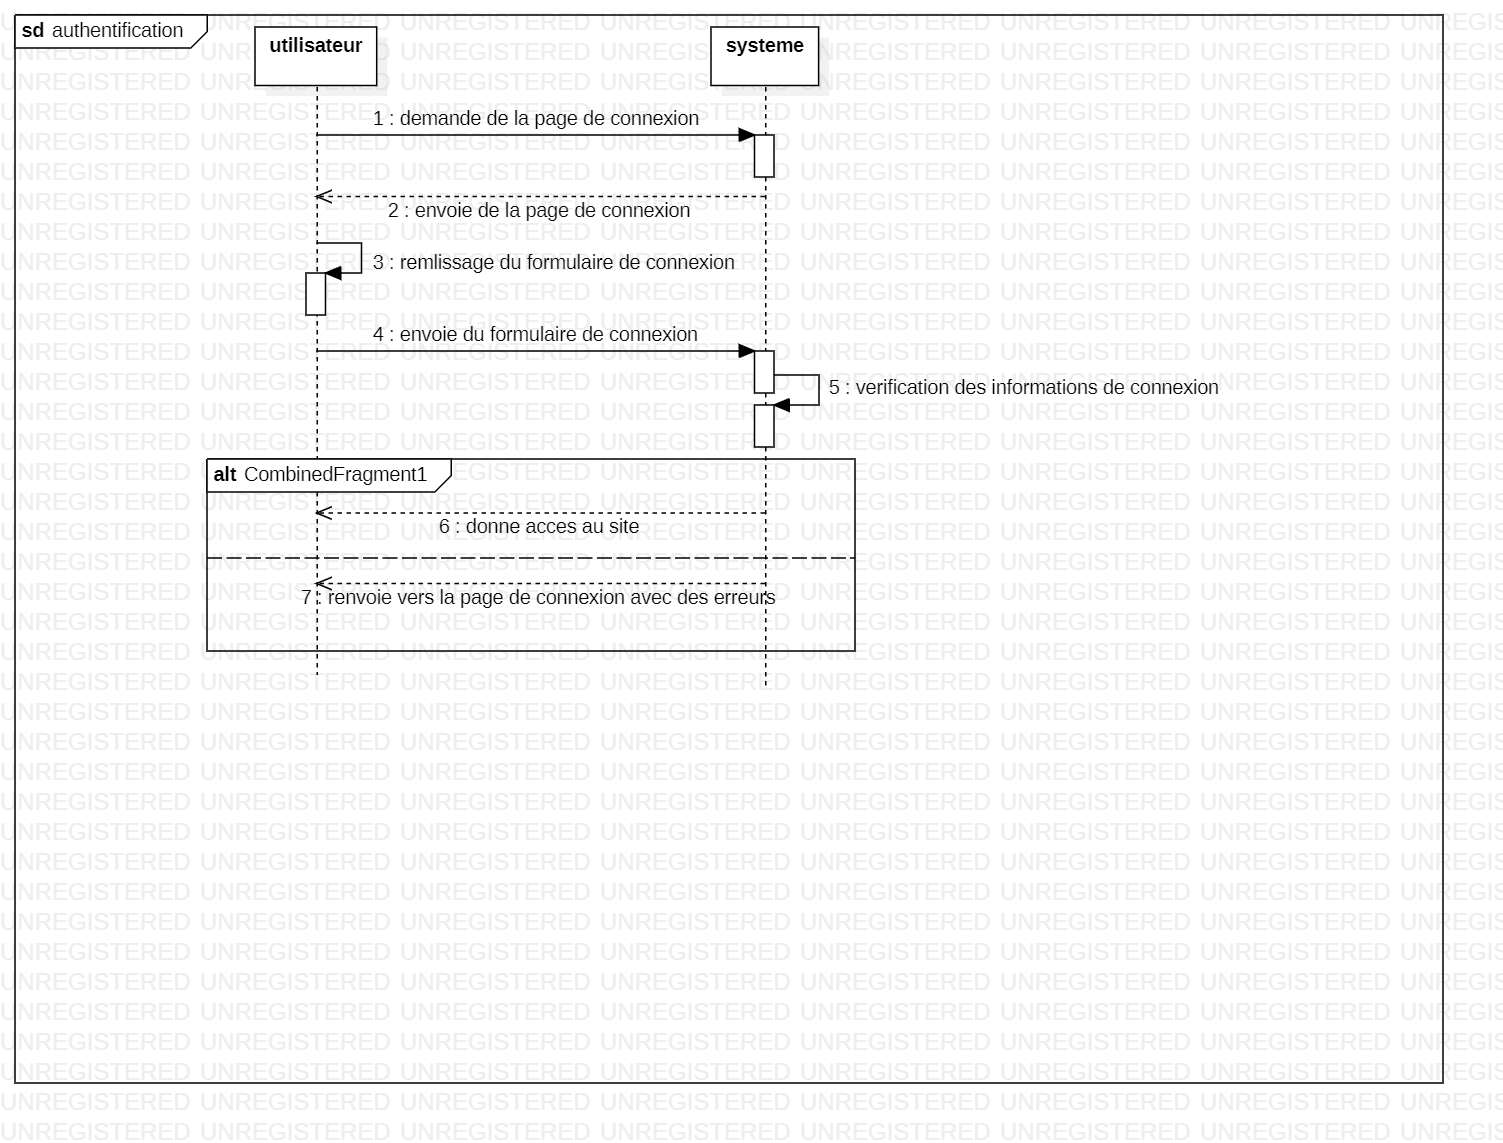
\includegraphics[scale=0.2]{img/authentification_seq}
 \caption{Cas d'utilisation general}
 \end{figure}
 \end{center}
 \subsection{Gerer les utilisateurs}
 \begin{enumerate}
 \item Creation d'un utilisateur
 \item Suppression d'un utilisateur
 \end{enumerate}
 \section{Diagramme de Classe}
\chapter{Resultats et Commentaires}
\chapter*{Conclusion et perspectives}
\end{document}